\documentclass[../HFT-main.tex]{subfiles}
\begin{document}
\clearpage
\section{\huge Rethinking Datacenter Management}
%
%Æthernet expects no predefined topology.  Every node (IPI Cell) has 8 bidirectional ports that connects to neighbors.
%
%==============
%\input{Document_Header}	% Bring in Paul's headers based on Memoir Header

%%\titleformat{\section}[block]{\color{blue}\Large\bfseries\filcenter}{}{1em}{}
%\titleformat{\section}[block]{\Large\bfseries\filcenter}{}{1em}{}
%\titleformat{\subsection}[hang]{\bfseries\filcenter}{}{1em}{}
%
%\renewcommand{\thesection}{\arabic{section}}											% Redefine Section numbering from rmp standard
%\renewcommand{\thesubsection}{\arabic{section}.\arabic{subsection}}						% Redefine Section numbering from rmp standard
%\renewcommand{\thesubsubsection}{\arabic{section}.\arabic{subsection}.\arabic{subsubsection}}	% Redefine Section numbering from rmp standard
% 
 % TELL THE STORY.  Non judgmentally.   Two separate tasks - get the thoughts down first, then make them readable (Steven Pinker).  Be concrete and visual.
 
% \begin{document}
%\section*{\fontfamily{phv}\selectfont{\huge{\bfseries{Rethinking Datacenter Management}}}}
%\section*{Rethinking Datacenter Management}
% \section{Paul Baran}
%
%\section{The Paul Baran Model}
%
%\subsection{Baran Centralized}
%
%Everyone recognizes the main disadvantage of centralized systems. As Paul Baran showed, they represent single points of failures and bottlenecks which prevent scalability. 


\vspace{-15pt}


%\subsection{References}
%
%\footnote{\href{https://www.rand.org/pubs/research_memoranda/RM3420.html}{Paul Baran "On Distributed Communications}}

%\end{document}

\begin{framed} 
\noindent Owners and operators of the network determine the relationships among distributed applications today. %, not by application developers.
Minimum spanning trees, on which all routing is done, are built, and torn down, by \emph{switches}; based on protocols standardized long ago when we first learned how our computers could communicate. %Allowing developers to build and manage their own routing substrate under API control would dramatically improve the performance and efficiency of modern infrastructures. 
%configuration, resilience and security of today's datacenter infrastructures.
\end{framed}
\begin{marginfigure}
  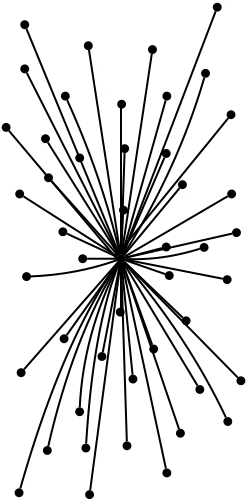
\includegraphics[width=0.6\linewidth]{../figures/Baran-Centralized.png}
  \caption{CENTRALIZED}
  \vspace{12pt}
\end{marginfigure}

%\section{Full Baran Set}
%
%\subsection{Baran Distributed}

\begin{marginfigure}
  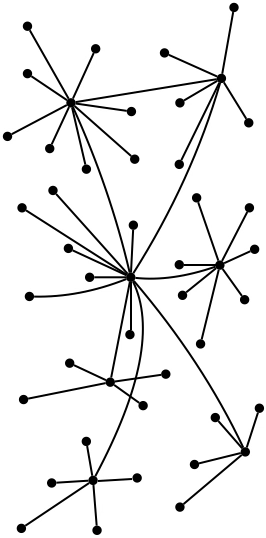
\includegraphics[width=0.6\linewidth]{../figures/Baran-Decentralized.png}
  \caption{DECENTRALIZED}
    \vspace{12pt}
\end{marginfigure}

%\section{Baran Evolving}

%\begin{marginfigure} % This is probably superfluous in this description 
%  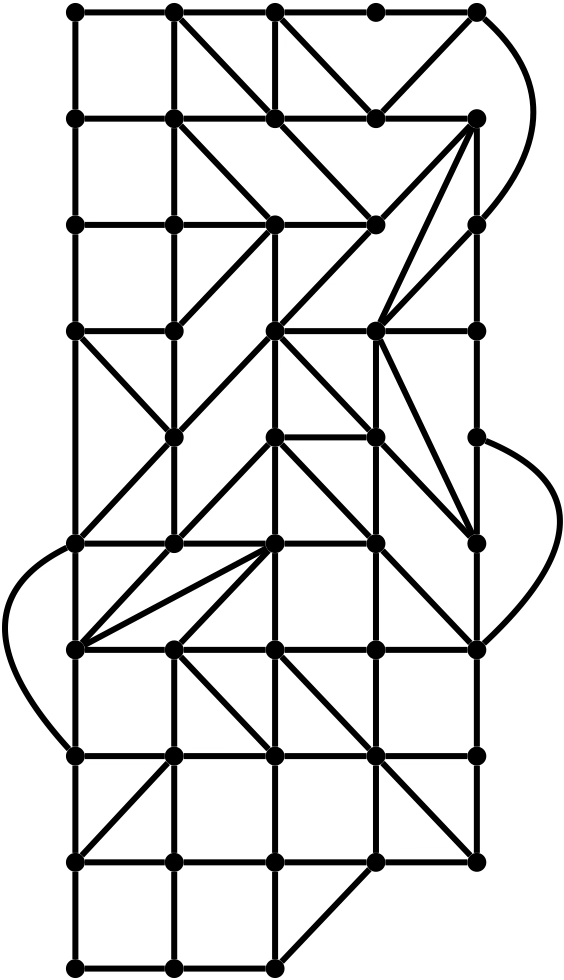
\includegraphics[width=0.6\linewidth]{../Figures/Baran-Evolving.png}
%  \caption{Baran Evolving}
%\end{marginfigure}

%Modern Clos Networks look like Decentralized Baran Networks.

%\subsection{Baran PNP}

%Partial Network Partitioning is a primary problem in the decentralized Baran Network


%\section{Baran Distributed -- Valency 4}

\begin{marginfigure}
  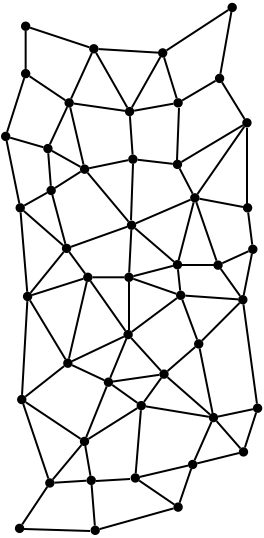
\includegraphics[width=0.6\linewidth]{../figures/Baran-Distributed.png}
  \caption{DISTRIBUTED}
    \vspace{12pt}
\end{marginfigure}
 
Today's datacenter architects build their infrastructures using two kinds of boxes: \emph{switches} and \emph{servers}.

We refer to all network devices as switches. Those that route at layer 3 are simply layer 3 switches.
%\footnote{There are also many hybrid kinds of boxes, often labelled as \emph{appliances}, such as \href{http://research.google.com/pubs/pub44824.html}{load-balancers}, firewalls, etc. These are often servers in disguise.}. 
They connect them using individual cables, which they bundle together to make them convenient to route within and around physical structures. This forms a \emph{centralized} or \emph{decentralized}% \footnote{In Paul Baran's terminology (\href{http://www.rand.org/about/history/baran-list.html}{Distributed Communications}).} 
 topology, where the switches become hubs and servers become leaves.
 
\noindent \href{http://www.rand.org/about/history/baran.html}{Paul Baran's classification} %scheme 
provides insight:\\ \texttt{CENTRALIZED (A)} shows 46 univalent nodes connected to a %47$^{th}$ 
special high radix or \emph{valency}

We use \texttt{valency} to denote the number of physical ports on a hyperconverged \texttt{cell}. A \texttt{cell} is a single type of node element (autonomous unit of compute, storage and packet processing). 

A \texttt{link} is an individual, bidirectional, computation object (an autonomous communication entity between  \emph{two} \texttt{cells}) This is to distinguish us from radix, used in switches, but is equivalent to degree ($\delta$), in graph theory.

If the central hub dies, all nodes are cut off.  \texttt{DECENTRALIZED (B)} shows 47 nodes and links, 7 nodes with a valency of  5-7 serve as switches, and 40 as univalent (leaf) nodes. If one of the switches fails, the network fractures into isolated partitions; and only nodes within the partitions can continue to communicate locally. \texttt{DISTRIBUTED (C)} shows 47 identical, multivalent (valency $\sim5$) nodes, and 98 links. The network has better resilience:  failed nodes are routed around, and many links must fail before \emph{any} node is finally isolated.

%How did we get into this mess?  TCP hides so much. 
\vspace{-8pt}
%\subsection*{Desirable \& Undesirable Topologies}
\subsection*{Datacenter Topologies}
%We all know that 
\texttt{CENTRALIZED} topologies are avoided because they represent bottlenecks and have a single point of failure. %  (SPoF's). %, so lets not talk about them anymore. 
\texttt{DECENTRALIZED} topologies are (hub \& spoke) topologies may be economically necessary for large-scale geographically disparate systems like the interstate roadways and airline networks. are  
most prevalent,  which is surprising given how \emph{non-optimal} they are  when looked at
from a perspective of distributed microservices container life-cycles

 Distributed microservices have an overwhelming predominance of East-West Traffic.  Containers can be created in microseconds and last only seconds or milliseconds.
 

 
 \begin{marginfigure}
  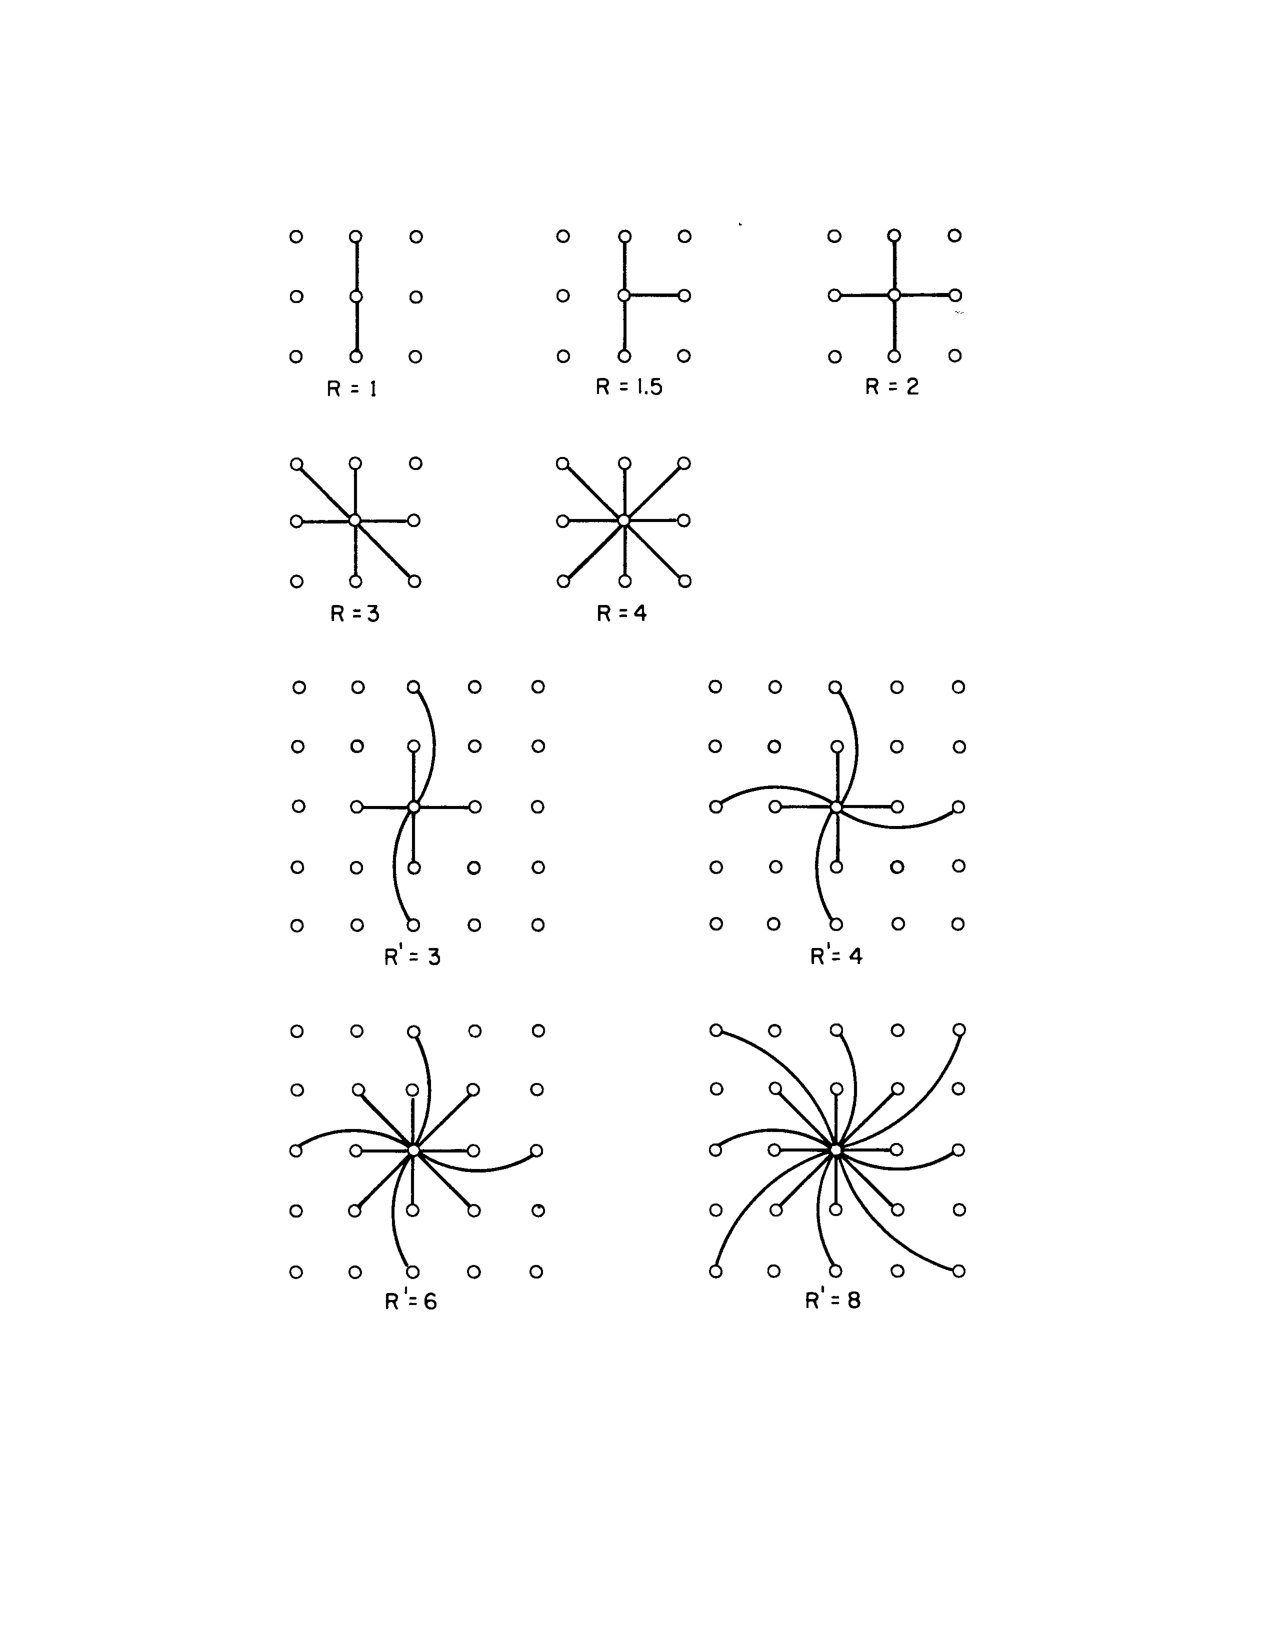
\includegraphics[width=\linewidth]{../figures/Baran-redundancy.pdf}
  \caption{Baran: Definition of Redundancy Level}
    \vspace{12pt}
\end{marginfigure}

 
 \begin{marginfigure}
  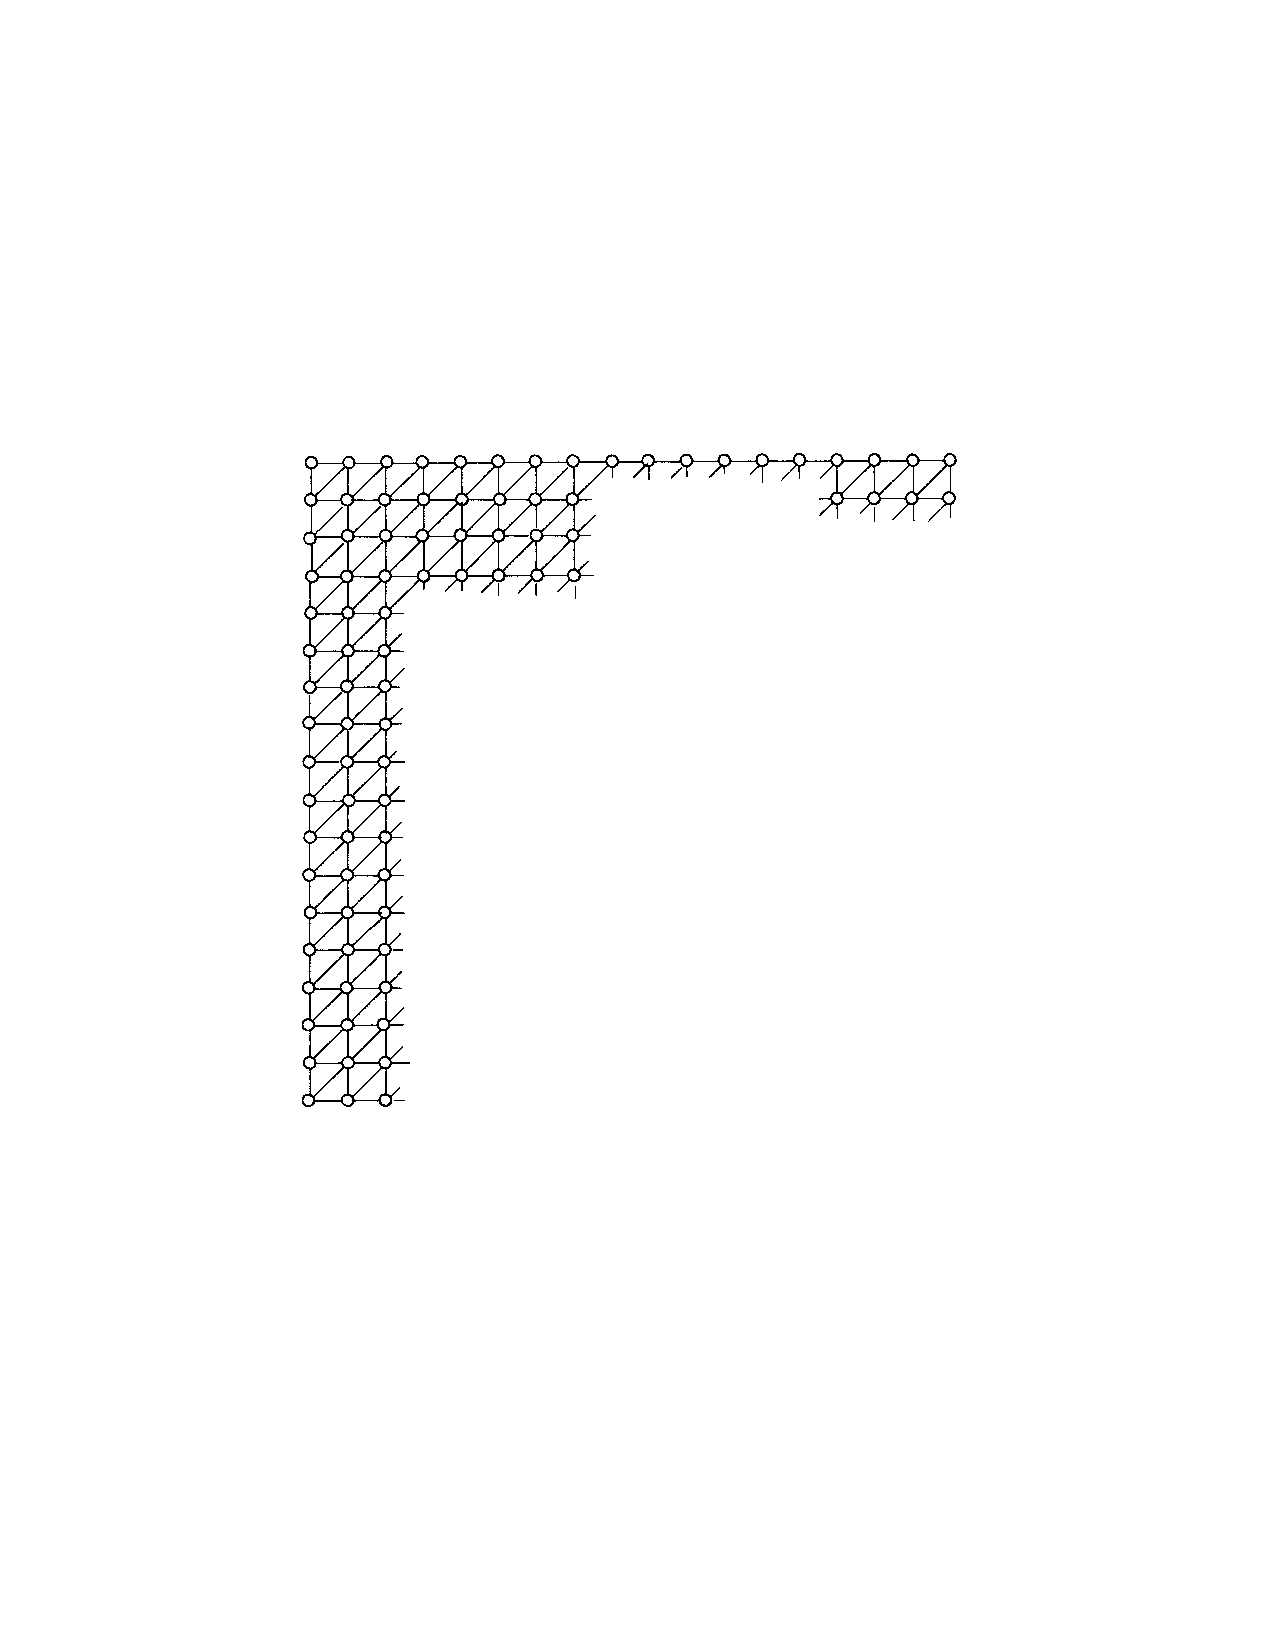
\includegraphics[width=\linewidth]{../figures/Baran-stations.pdf}
  \caption{Baran: Array of Stations}
    \vspace{12pt}
\end{marginfigure}
 
 
 %migration, elasticity and resilience

Today's datacenter networks evolved from their roots in the ad-hoc connection of Ethernet broadcast domains with switches housed in wiring closets and managed by individuals with specialized expertise in routing and proprietary management interfaces.

 The SPoF's in decentralized topologies are mitigated by redundancy in modern multi-slice Clos Networks. Modern Clos networks typically have two, three or four \emph{slices} of spline and leaf switches, along with multiple sets of cables..
Switches  networks that perpetuate this model, are embarrassingly complex, unreliable, arcane, and parochial. This results in very high operational costs, poor security/high vulnerability, and nothing close to five nines reliability
 [{From \href{https://www.linkedin.com/pulse/why-network-industry-has-been-stuck-1980s-ciscos-embrace-joe-howard}{Joe Howard}, The perpetuation of complexity:
 
 
\begin{quotation}
\noindent  ``Ethernet and IP networking is embarrassingly complex, unreliable, arcane, and parochial. That results in very high operational costs, poor security/high vulnerability, and nothing close to five nines reliability. In almost any other product category this would be considered unacceptable. Network technology has changed very little since the late 1980s, with the exception of faster speeds/feeds and some additional protocols and features.''
\end{quotation}}

% In almost any other product category this would be considered unacceptable. %Network technology has changed very little since the late 1980s, with the exception of faster speeds/feeds and some additional protocols and features.''
%
\texttt{DISTRIBUTED} topologies are rarely used (so far) in datacenters, except for a few HPC applications. Except for HPC applications, which have used various forms of hypercube routing, based on a cartesian coordinate system of destination addresses (a God's-Eye-View), which assumes that failures are rare, and uses complex band-aids to route around failed nodes. 

When we use a \emph{relative} addressing scheme instead, routing around failed nodes becomes far simpler, and we can build entirely new kinds of stacked graph covers to provide functionality not previously needed (or envisaged) on hypercube interconnects.. 

However, within the same \emph{or lower} capital~cost, \texttt{DISTRIBUTED} topologies provide: greater resilience, lower latencies, higher available bandwidth and far more flexibility; by connecting \texttt{cells}

We combine switches and servers, into a single concept:  \texttt{cells}, and make them \emph{substitutable (i.e. although they may not be identical in all aspects of their capabilities, they can at least be managed as one `type'.), which, in turn, makes them \emph{fungible}, and easier to manage. The additional density of the physical topology, afforded by the \texttt{cell}'s  `middle' range valency ($5$ to $9$), enables far richer virtual topologies to be built.} directly with neighbor to neighbor (N2N) %or directly-connected arrangement
connections rather than through a switched or \href{http://www.plexxi.com/2013/07/the-problem-with-everything-in-aggregation/}{aggregated} network. By not perpetuating the management complexity of switched networks, and introducing new, simpler, control/forwarding planes through \texttt{cells}, we can also dramatically lower  operational costs. 

%\footnote{This allows us to avoid almost all the problems of todays networks caused by the \href{http://www.plexxi.com/2013/07/the-problem-with-everything-in-aggregation/}{\emph{aggregation mindset}}. Just as with the naysayers in Paul Baran's time, skeptics today will often invoke \emph{argumentum ad ignorantium} (arguing that a proposition is true because it has not yet been proven false (or vice versa).  When pressed they will often fall back to the argument that: ``we've always done it this way'', or, ``it must be legacy compatible'', etc.  We contend that modern datacenter networks can gain significant advantages by adopting Paul Baran's \emph{fully distributed} model. This may not have been obvious in the past because networks were relatively static, and security was not considered a particularly important problem.}. 
% Dense networks represent an opportunity that has so far been overlooked by datacenter architects.


%Additional state stacked on top of the  \texttt{links} in TRAPHs are lost, or at least made so \emph{uncertain} we have to start again from scratch to rebuild them. Applications have to watch out for themselves, networks don't persist state. This forces ALL communications into the \emph{list} model instead of the \emph{graph} model. TRAPHs are thwarted at every turn; any graph structures they build are demolished every time a switch hiccups. %burps, farts or shits itself.

\vspace{-2pt}
\begin{framed}
\noindent Perhaps the time has come to recognize the genius of Paul Baran's insights, and ask why \texttt{DISTRIBUTED} topologies are not deployed in datacenters, where their resilience and security can be readily exploited?
\end{framed}
\vspace{-16pt}
\subsection*{Datacenter Programmability}
\vspace{-4pt}
Two types of teams co-evolved to manage modern datacenters: one to design and manage the networks, and one to program and manage the servers. This worked % \emph{OK}% for  years,
when datacenters had a single owner or tenant, their applications and physical infrastructure evolved slowly, and different business units could work within their own silo's. % to optimize their business purpose. 
This is no longer a viable architecture in today's highly dynamic multi-tenant datacenters.
\vspace{-3pt}
\begin{framed}
\noindent Distributed applications can no longer afford to be held back by the slow pace of networking innovation.
\end{framed}
% FROM ALAN: I don't see how distributed applications are being held back by the slow pace of network innovation.


%\subsection*{SDN: Programmable Networks}
%The industry's response %to the slow pace of networking innovation
%has been to introduce %the notion of 
%Software-Defined Networking (SDN) to  program networks. % behavior. 
%But SDN is  (a) \href{http://etherealmind.com/sdn-is-not-an-innovation-its-iteration/}{incremental} and (b) its \href{http://forum.stanford.edu/events/2016nickmckeowninfo.php}{programmability} continues to be confined to the \emph{network control plane}; which remains under the control of network owners and operators.
%
%High-performance forwarding chips based on PISA (Protocol Independent Switch Architecture)
%%\footnote{PISA is Protocol Independent, it allows \href{http://p4.org/spec/}{P4 programs} to specify forwarding behavior for packets. It is suitable for describing everything from high-performance forwarding ASICs to software switches. Field reconfigurability allows network engineers to change the way their switches process packets after they are deployed.} 
%can be programmed by the \href{http://www.sigcomm.org/sites/default/files/ccr/papers/2014/July/0000000-0000004.pdf}{P4 language}. While this is a step in the right direction, it is too low a level of programmability
%%\footnote{P4 presents a paradigm of ``programming with tables'' to developers. This paradigm is somewhat unnatural to imperative (or functional) programmers, and it takes some time to get accustomed to the abstraction. It also, occasionally, leads to awkward ways of expressing functionality [\href{http://arxiv.org/abs/1511.04985}{Paxos Made Switch-y].}}, 
%supporting the conventional notion that switches \emph{forward} packets to \emph{destination} addresses.
%
%%\footnote{In P4, programmers declare how packets are processed, and a compiler generates configurations for a protocol-independent switch or NIC. For example, network programmers can program the switch to be a top-of-rack switch, a firewall, or a load-balancer; and add features for monitoring or automatic diagnostics.}. 
%

While programmable switches may be a promising approach to improve the performance and manageability of datacenters, they are still (a)  under the control of the network owners and operators, and (b) limited by the low-level endpoint routing and packet forwarding paradigm of today's network engineering. What is needed to complete this revolution is to include the cells (agents on servers) as first class members of this set of devices which are allowed to route packets as well as process them.

\vspace{-8pt}
\subsection*{TRAPHs: Programmable Application Topologies}
 
Critical layers are missing between applications and infrastructure: a layer which contains the evolving \emph{graph} relationships of modern microservices. A substrate that  programmers can own and manage themselves\footnote{A substrate that can work in conjunction with the simpler forwarding functions within NICs and switches}.
This provides the missing abstraction for a programmable, and deterministic-when-needed, topologies as tools and resources to the application architect. For example, application programmers can program these TRAPHs (Tree gRAPHs) using a Graph Virtual Machine (GVM) to provide services such as distributed consensus, atomic broadcast, and presence management among members of a cluster or microservice set. %We already have network nodes in hosts (e.g. vSwitches)

TRAPHs enable datacenter operators to organize \emph{graphs} of resources, managing them on trees, enabling computing on graphs. From the perspective of different vantage points, each with least-privilage\footnote{E.g. Managing realms, jurisdictions, tenants and sub-tenants as graphs instead of lists.}. They also provide developers of microservices complete freedom (within the nodes assigned to them), to programmatically determine their sub-relationships, and the protocol characteristics most needed for their applications.
\vspace{-16pt}
\subsection*{Examples}
\vspace{-2pt}

The advantage or using TRAPHS over a distributed network is that application developers can program their behavior instead of having to wait for permission, or suffer the externalities of the network optimizing itself without regard to the application's health. This simplifies some important use cases such as:
\begin{description}
	\item [Logical \& Virtual Segregation Planes] Enable capability-based security graphs, to provide secure containment of communication environments for multi-tenant infrastructures. E.g., exchange the management of lists (ACL's and \texttt{iptables}) by replacing them with richer and more manageable \texttt{graph equations}. Virtual Segregation Planes: graph applications: erasure coding, machine learning, etc.
\vspace{-3pt}
	\item [Coherent graph overlays] where cache \emph{heterarchies} co-exist to automatically manage the placement and eviction of caches based on request patterns. One use case would be a coherent configuration file system, which provide a unified mechanism to keep configuration files synchronized, for Docker, etc. Another would be a \emph{coherent} \texttt{memcached}. Eliminating \href{https://status.cloud.google.com/incident/compute/16007?post-mortem}{cascade failure incidents}, like Google saw recently spread to all regions of their Cloud Platform due race conditions to update configuration files. 
\vspace{-3pt}
	\item [Managing Infrastructure as Sets, Graphs \& Tensors, \emph{instead of} Boxes, Files \& Lists.]  All routing is predicated on building shortest path trees, e.g. Bellman-Ford for L2, or Dijkstra at L3. The roots for these trees are in the switches, and thus under the administrative control of network owners and operators. With TRAPHs, large subgraphs, or graph-covers comprising \texttt{cells} and \texttt{links} allocated to a particular tenant, may be used by that tenant for any topology whatsoever, including allocation to sub-tenants. \emph{Graph computing} on TRAPHs (Tree-gRAPHs) enable automatic mapping of the natural DAG relationships of distributed applications on  nested % (physical, logical, virtual)
datacenter infrastructure resources.
\vspace{-6pt}
\end{description}
\vspace{-6pt}
\begin{framed}
\noindent \textbf{Conclusion:} Allowing application developers to build and manage their own routing substrate under API control would dramatically improve the performance, efficiency and flexibility of modern   infrastructures, reducing inter-tenant interference, enabling privacy, and improving manageability.
\end{framed}

%Allowing application developers to participate in the setup and tear-down of dynamic topologies, would result is a datacenter fabric that is simpler, more resilient, easier to manage, lower cost, more secure and fundamentally more recoverable.
 
\section{The Evolution of Baran to Chiplets}

\begin{marginfigure}
  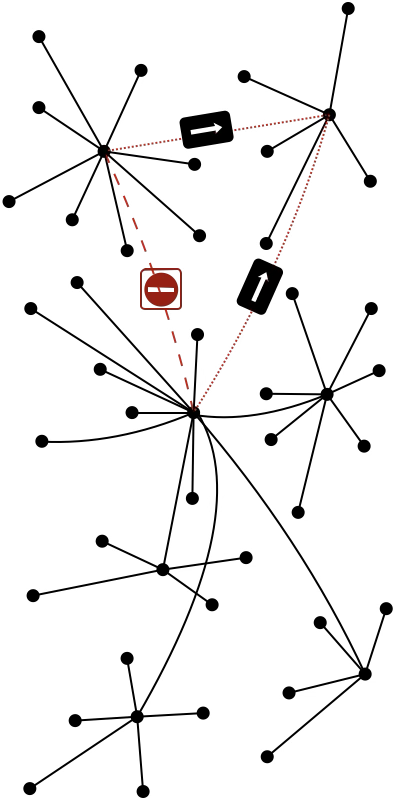
\includegraphics[width=0.6\linewidth]{../figures/Baran-Decentralized-PNP.png}
  \caption{ Partial Network Partitioning}
  \vspace{20pt}
\end{marginfigure}


\begin{marginfigure}
  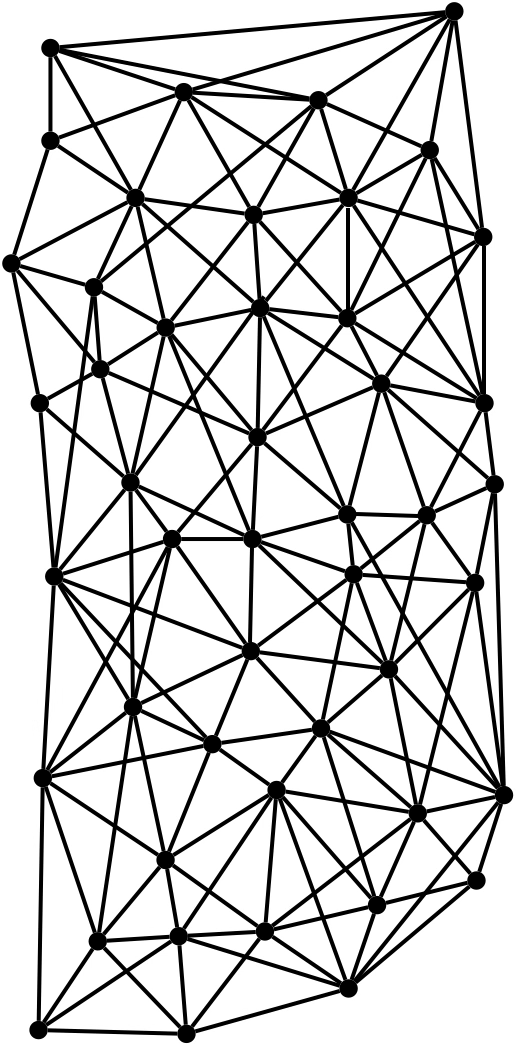
\includegraphics[width=0.6\linewidth]{../figures/Baran-valency-8.png}
  \caption{Distributed (valency 8)}
    \vspace{20pt}
\end{marginfigure}

  
\section{Baran Distributed}

\section{Baran Chiplet}

\begin{marginfigure}
  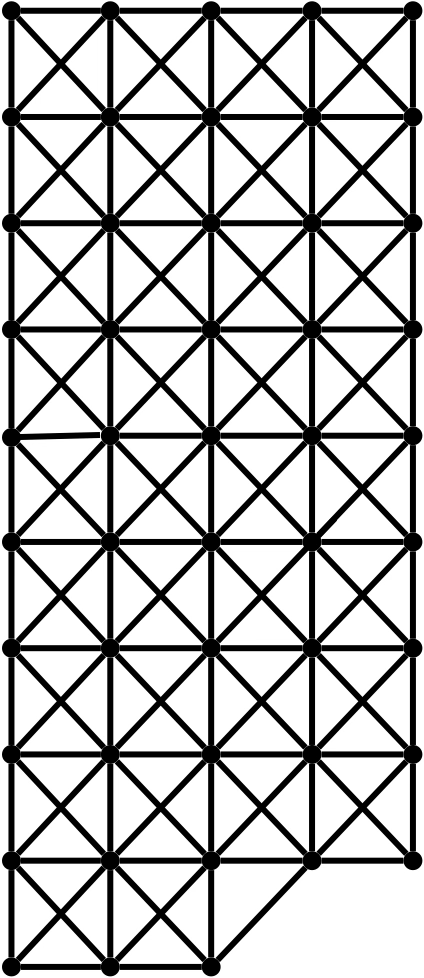
\includegraphics[width=0.6\linewidth]{../figures/Baran-Chiplet.png}
  \caption{Baran Chiplet}
    \vspace{20pt}
\end{marginfigure}

\clearpage

\end{document}


%  ladder diagram that outlines the flow of information? 

%\newpage
\theendnotes


%%\input{TRAPH}
%[Eliminate Unnecessary Contention] e.g.  The \href{http://ieeexplore.ieee.org/xpl/articleDetails.jsp?reload=true&arnumber=6762979&abstractAccess=no&userType=inst}{TCP incast Problem}\footnote{See: http://www.pdl.cmu.edu/Incast/}. 
%\noindent Our goal is a fundamental redesign of datacenter fabrics. ; 

%Key innovations include a \emph{logical control plane} (to enhance manageability), \emph{serialization foci} (to enhance resilience and serializability), and a \emph{virtual data plane} with an integrated
 % \texttt{crdt}'s 
%\emph{metadata tensor} (to enhance consistency and recoverability); all based on a significantly improved \emph{model of time} which enables a dynamically deterministic ordering of events as a controllable (programmable) resource for distributed systems services supporting consistency, coherence, consensus and recovery.

%We seek to address fundamental customer pain points in resilience, security and manageability of \emph{configuration data} (little data) as systems scale, from the small, to the very large. Our plan is to introduce three compact low level mechanisms that enable distributed systems to be deployed quickly and easily on virtual infrastructure, and most importantly, have fast recovery capabilities in the face of perturbations (reconfigurations, failures, disasters, attacks): %Our vision is an open platform for graph computing. Our target market is cyber-defense.  For datacenters of all varieties and scales, everywhere.
%RAFE (Reliable Address-Free Ethernet ),  (AIT) Atomic Information Transfer and TRAPHs (Tree gRAPHs).


% \href{http://packetpushers.net/the-sad-state-of-data-center-networking/}{The sad state of datacenter networking.}

%\end{document}
\clearpage
\section*{Additional (unformatted) notes}

% Notes from Cumulus Seminar. 

\subsection{Bridging}

Most datacenter operators today are considering building networks using  Layer 3 for everything. Some think about using VxLAN, but in general, L3 is beginning to dominate how.

Applications and servers are the last bastion of bridging.

Application designers: 
Service or node discovery relies on broadcast.  This implies assumptions about being in a single subnet. The assumption is built into the application that everything is bridged.

 Cluster heartbeat uses multicast.  This again assumes a single subnet, because L3 is seldom used. 
 
VM mobility continues this trend.  These are examples of how applications are designed and as a result, prevent applications being scalable.

Previously, L3 was slow and expensive.  Vendors charged extra for L3 licenses on the same box, and yet another expensive license for BGP

There is no good routing protocol stack on the host!!   L3 is considered complex to configure, and L2 is considered easy, although that is mythical because it was just plug and play.

New silicon from Broadcom, Cavium, Mellanox.  Merchant switching silicon can perform bridging and IP routing at the same performance and price.

Open Networking solutions such as Cumulus Linux offer routing at the same price point as bridging.

Routing on the host:  Cumulus Quagga.    \href{http://bird.network.cz/}{BIRD} ?   \href{https://github.com/Exa-Networks/exabgp}{ExaBGP}.  (Exa-Networks is the swiss army knife of networking).
Windows Server 2012 also has BGP built in.

OSPF unnumbered, BGP unnumbered. ??

How are modern applications designed for a pure L3 network?   Kelsey Hightower

Kubernetes.  Manages applications. Packaging applications in standard containers and use automation tools to push them around on an infrastructure. Everything at Google runs in a container.  Even the VM's run in a container.  Containers are replacements for rpm's , tarballs. jar files, etc. Manage applications, not machines.

MASTER: Everything in Kubernetes is declarative.  to run a container, have to declare the state.

Nodes - Kublets.

API will automatically manage the entire cluster rather than the individual nodes 

Use for : Workload portability.   WORA.  Goal - avoiid vendor lock in.   Runs on GCE, AWS, etc.

Goal Avoid coupling. Dont force apps to know about concepts that are Kubernetes-specific.
Examples: namespaces, Services/DNS
Not guaranteed to have the same identity.  Cant rely on an IP address 
Instead, 

Pods = lowest level primitives in K.  Key to understanding.  A collection of one or more containers ALONG WITH THEIR VOLUMES.
Things that need to be scheduled on the same node.

Can die, cannot be reborn with the same ID.  Very similar semantics to VM's.

Most apps require some kind of volumes.   empty dir, tempfs, Host path, Git repository, GCE persisent Disk, AWS EBS, Azure, iSCSI, Flocker, NFS, GlusterFS, Ceph File and RBD, Cinder, FibreChannel, Secret, ConfigMap, DownwardAPI, Flex ...

Replication controllers control loop. Scan cluster through API and determine if containers are still running.  Start with 1 pod, define can run say 4, once 4 is up and running.  The replication controller will make sure 4 are always running.

Deployments provide updates as a service. Rolling update is imperative, client side. 

End to end, registered with underlying load balancers.   Program to the kubernetes API, build any automation you want.

Namespaces. A way to partition cluster by organization, users, etc.  Slice up cluster into quotas.  Key to doing policy enforcement.
Prevents one set of apps in one namespace from 

More of a logical partitioning.  A way of isolating things; group A, Group B, etc. Inside Kubernetes.

Kubernetes Networking Model. Understand how simple it really is.

Familiarity with Docker Networking.   Each node has a private network of its own (IP addr), and exposes services by doing some kind of NAT translation outside the machine. Most people do this with port mapping. The app uses one port, then map to a high level port that didn't need to tell other applications about.

This gets really messy really fast. You now no longer have a 1:1 translation, for  SQL DB on port 3306 (internally on one container) is now presented to other machines on port 9376.  Causes confusion for 

Now need service discovery, when not quite sure what port and IP will be.   Get port collisions.  A big problem, especially at larger scale. Very prevalent in the Java -- e.g. port 8080.

	REJECTED (ABOVE).
	
QoS, Latency and Jitter? Does K allow you to specify those 

K uses underlying runtime to use cgroups allows us to do things at very low level of networking.  
uses for memory, ram, disk, Goal: manage every resource.  Describe those resource allocations and enforce them.

** Currently: network I/O is TOUGH **

Kubernetes Networking Model:  Key - one IP address per POD.  These IP addresses are first class citizens in that pod.

IPs are routable (vs docker default private IP 
Pods can reach each other without NAT. Even across nodes.
No brokering of port numbers. too complex, whiy bother?
THIS IS A FUNDAMENTAL REQUIREMENT:
Can be L3 routed.
Can be underlayed (cloud)
Can be overlayed (SDN)

You can have multiple copies of your applications running on a single server and avoid port collisions, even across multiple nodes.

Today - start with docker bridge, assign \\24 network - provides 250+ hosts on a single machine. Allows multiple copies on single machine.

Most people reach for an overlay between boxes.  But there is a huge performance hit !

Dinesh question - how do you enable a view of real time (e.g. IEEE 1588 applications).

Answer - lowest level, physical world.  Routers, F5 balancer. 

Cluster management - real time interface for global time is OUT OF SCOPE for KUBERNETES.  K only cioncerned with deplooy and igivng resource allocations. Giving a dif

Real-time time services True Time could in theory run on top of Kubernetes.  Pattern: addon:  DNS< loging, monitoring, take very popular open source services and 

Not shipped by core Kubernetes out of the box.

Dinesh. The machine need to keep real time. 

Kelsey - Distributed systems are hard, even beyond that, time synchronization is hard. All kinds of way of doing it.  Logical clocks.  Manage lotica

if use something like google true time.   OUT OF SCOPE FOR TODAY.

Kubernetes model:

Once we've allocated a subnet PER HOST. i.e. given a slash 24 to each host. 

Can talk to any other pod in the cluster, can talk to any other container within each pod or host.

The do not enforce how they route, nor do they enforce L3 !!  You are free to bridge the private network.  Not good for scaleability.

Network Isolation: Describe the DAG of your app, enforce it in the network. 

Restrict Pod-to Pod traffic, or across Namespaces.

Designed by the network SIG
- implementations for Calico, OpenShift, Romana, OpenContrail (so far).
		Status Alpha in v1.2, expect beta in v1.3  

% This is closest to what we are doing in TRAPHs

USING A NAMESPACE TO CONTROL WHAT PODS CAN TALK TO WHAT OTHER PODS.  

Dan do this because can have containment based on application boundaries.

Within each pod 

Allows us to have on IP address, and one networking stack per container group. Can expand this across network namespaces. (Kubernetes Namespaces).

[PN - see snapshot of screen - very good figure showing isolation - cut this out and show comparison for competitive analysis]

 Project Calico allows you to have network relationships driven by namespaces.  Handy for people who are looking for more granularity than is provided by Kubernetes out of the box.
 
 NETWORK PLUGINS
 	VERY Experimental
	
 Using a standard network plugin called CNI (CoreOS) in v1.1		Invented at CoreOS 1-1/2 years ago.
 	- Simple exec interface
	- NOT USING DOCKER LIBNETWORK - but can defer to docker for networking
	
	Cluster admins can customers their installs:   DHCP, MACVLAN, Flannel, custom

 CNI runs in a namespace to configure the network stack.
  
This is more than bleeding edge, can get fired for getting wrong.

SERVICES

Now have IP addresses for all Pod's.  How to get to the outside world.  By default have labels.

Services can be automatically integrated into Load balancer (eg. F5) up date back-end dynamically.

All this talk of SDN  (Spreadsheet Defined Networking).

Services are a group of pods that work together.
- grouped by a selector,
Defines access policy (load balanced, or headless)
Gets a stable virtual IP and port. Sometimes called service portal, also DNS name
VIP is managed by Kube-proxy
	- watches all services
	- updates iptables when backends change
	
	Hides complexity - ideal for non-native apps.
	
Round robin around all pods that make up the service.

Can reference any other service ON THAT CLUSTER

Ip tables:

Kube proxy runs on every server. Interfaces with iptables. 

A separate apiserver. 

kbectl run. (gets IP addresses of each back end pod)

kubecel expose.  (expose IP address to outside world.

updates IP tables,

Random algorithm in iptables will find endpoint. Gets even distributeion of traffic on each  machine.

Drawback -- have a double hop. no guarantee will stay on the same machine.

Services IP's are only available inside the cluster.

Need to receive traffic from the outside world.

Builtin - Service type, NodePort - expose port on every node.  Load balancer - provision a cloud load balancer.

DIY load-balancer solutions (socat - for nodePort remapping) ha proxy, nginx.

External services -enable to talk to load balancer.

Skipped over Invress(L7) 

Kubernetes handles multi-tenancy. Exposes some of security constructs. SELinux, 

Multi-tenancy - untrusted apps for multiple users, not supported today.  

RPM's jar files, multi tenancy today?  partitioning - Kubernetes - only run on certain machines.

Kubernetes is not the holy grail to run your mutlitenant cloud applications on.

Kubernetes is an easy way to deploy applications. e.g. manage and orchestrate. 

HOST CONFIGURATION ...

Ideally:

	neighbor eth0		[Peer with neighbor on eth0]
	redistribute connected		[and distribute my connected route]

In reality, a few more lines

	router bgp 65534
	bgp router-id 10.10.1.1
	neighbor eth0 interface remote-as external
	redistribute connected

Two ways to use bgp on the host:
 - use dynamic neighbors
 - use BGP unnumbered.

ToR is configured with subnet from which clients can connect.  Clients initiate connection.

Rest of operation is regular BGP

bgp listen range 10.0.0.024 peer-group SERVER bgp listen-limit 8

Connection to serves is not bridged, but p2p
	- pure L3
	
Interface-based configuration with remote as external.

Can also do it with OSPF

HOSTS ARE ALWAYS STUB NETWORKS, NEVER TRANSIT
- hosts are in separate area from rest of network with OSPF

Announce only default route to host 
Accept only specified prefixes from host.


Claims that high quality open-source routing stacks are available for hosts (Cumulus Quagga is one of them). 

%\clearpage
%
%\subsection*{Notes for Bill Vass}
%\begin{verbatim}
% Notes for Bill Vass
%	Two pager: pains and gains
% 	Key concerns:  Cost, Reliability (of the whole stack),,  Scalability,  OPEX.
%		FOCUS on plumbing -- network switches.
%	High Level, diagram(s)
%		Reliability
%		Scalabiltiy
%		Security
%		Data Transactions  (Massive Databases)
%
%	COST
%	Resiliency
%	Ability to provide low-cost storage.  Deliver more to more customers, at higher performance and lower cost.
%	
%		What will grow his business ?
%		What keeps everyone jumping on board @ Amazon
%		Keeping client customers happy
%			Secure, data, interconnect  (Ex Baracuda)
%		Network security @ NSA
%		Deliver more with less.
%\end{verbatim}


%The \emph{shared state} becomes a resource to facilitate recovery: dedicated to re-establishing communication, and when it heals, we carry on. If that \texttt{link} doesn't heal, the \emph{shared state} (atomic tokens) are preserved and returned back to the initiator. % on the next failover tree, %stitching the \texttt{link} \emph{shared state} back together again \emph{deterministically}.  %This recovery property can be composed into any arbitrary structures stacked on top. % of those links by any number of trees. % This is TRAPHs.

%	Bill C / Al S   1/2 page Pains & Gains then next level deep
% 	Go back to Paul Baran - time to bring all that to the Datacenter, for the reasons Paul Said.
% What's different:
%	(1) a link level protocol that gives certain characteristics we can build on.
%	(2) All DC's are deploying Applications.  Applications have structure, that structure can be deployed on top of this new architecture (with N2N links). so it can be deployed and grow organically using migration to scale (evolve with demand).
%Its time to explore plumbing computers in racks without switches (or soft switches). What's different  is:
%
%(a)  A link level protocol that gives certain characteristics for distributed systems that we can build on.
%(b) Distributed applications have structure; that structure can be deployed on top of this new architecture (with N2N links). so it can grow organically using migration to scale (evolve with demand).
%
%This solves complexity; not by managing it, but by replacing it with simplicity.  Re-evaluating the topology of connection allows us to address the impedance mismatch between the virtual (distributed application) topology and the physical (switched network) topology.  

%
%We start with networking
%We continue with little data 
%We complete with computation graphs
 
 
 \end{document}



\newpage
\section{Compass Point Scouting -- THIS IS IN TOPOLOGY.   Dup ?}
\begin{marginfigure}
  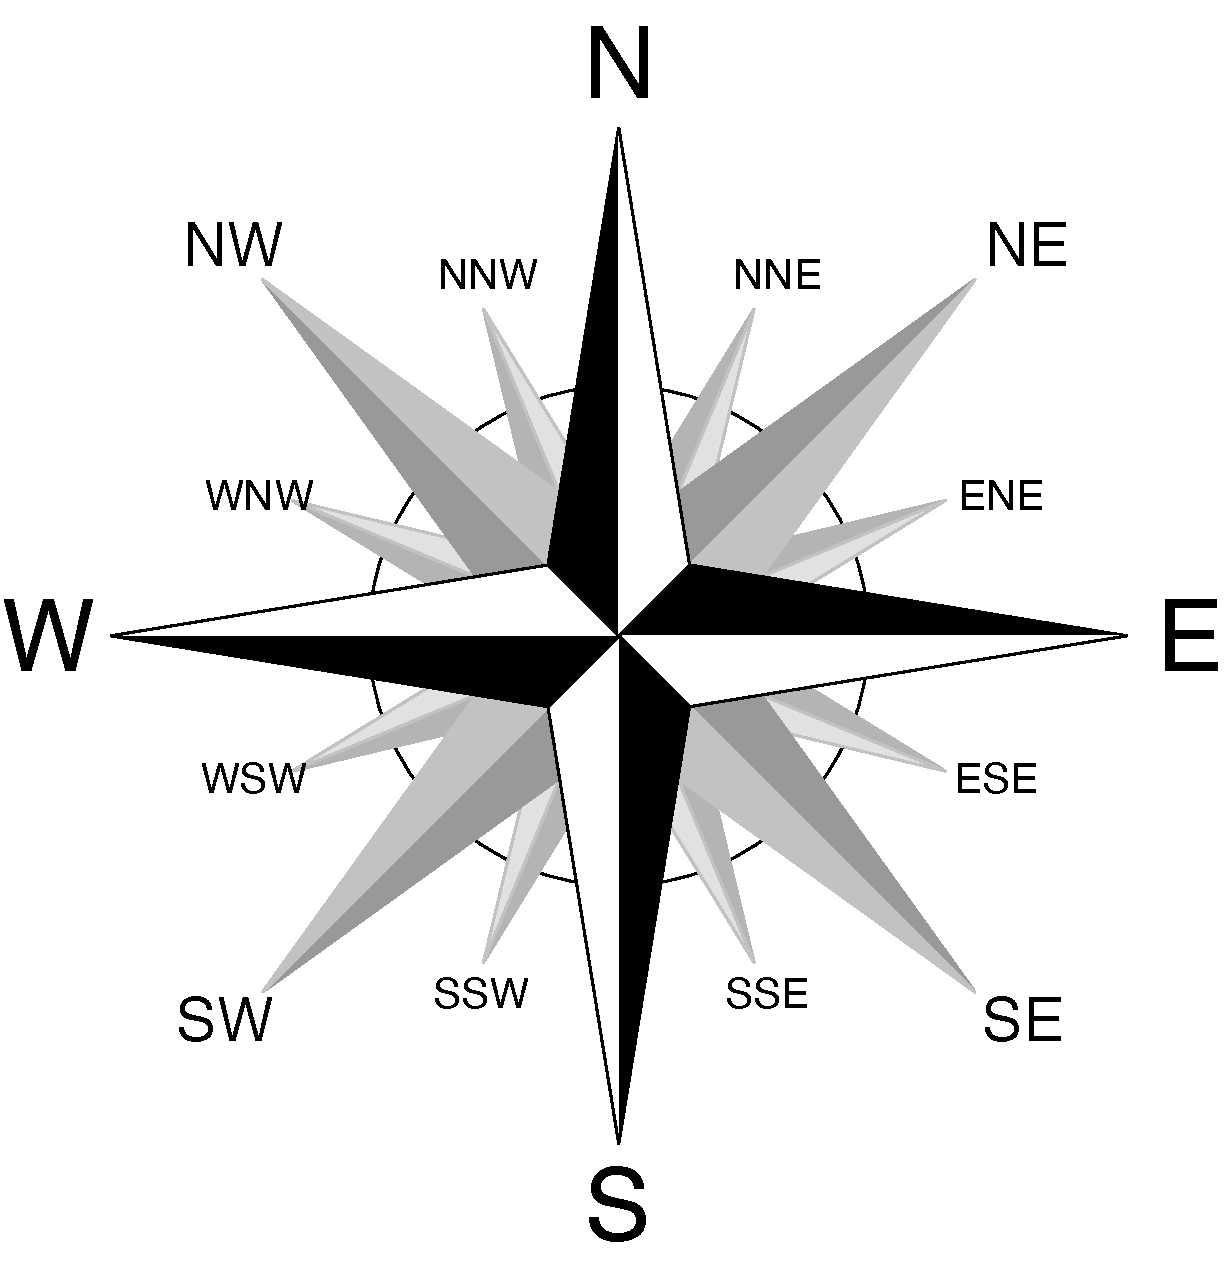
\includegraphics[width=\linewidth]{../figures/Compass-Rose.pdf}
  \caption{Cardinal and Intercardinal Compass Point Routing on 8-valency nodes with 16 possibilities for TX/RX channels on each port (direction)}
\end{marginfigure}

Every Cell (IPI/SmartNIC) with 8 ports  discovers its environment.

Each of these 8 ports has 2 connections (transmit, receive). Although the Chiplet Ethernet specification allows for initial configuration and reconfiguration of these to be used for other purposes, and for dynamic reconfiguration. 

We specify \emph{scouting} protocols as a precursor discovery protocol, and underneath \emph{routing} )dscribed later  

Because any absolute cartesian naming scheme cannot scale, is brittle (to errors and reconfigurations) we use a relative addressing scheme for the scouts (Ants, Bees), for each cell to independently discover its environment. 

Scouts  therefore use \emph{source} routing, where the path explored is pre-determined. As in the case of Ants, these directions can be random. They leave a pheromone trail so they can find their way back home.  In Æthernet clusters, Ants can have other kinds of exploratory behaviors, such always turning right or always turning left, to explore the neighborhood in a circular fashion. 

These kind of mechanisms have already been explored in the literature, and is known as deflection or bufferless routing. \marginnote{\href{https://citeseerx.ist.psu.edu/document?repid=rep1&type=pdf&doi=e367d9c8aa35ad1bfd4aa15c58723e84cae4a413}{A case for bufferless routing in on-chip networks. Thomas Moscibroda, Onur Mutlu}}
\cite{goyal_backpressure_2020}

\section{Connection with bufferless and deflection routing}

The next section is an overview of how biologically inspired ``scouting'' or ``discovery'' mechanisms connect with key ideas in bufferless (hot-potato) routing and deflection routing, especially in mesh-like topologies where routers have ports arranged along the cardinal (N, E, S, W) and intercardinal (NE, SE, SW, NW) directions. Although the terminology and details vary across papers, the essential themes can be traced in both NoC (Network-on-Chip) and larger-scale interconnection network literature.


\subsection{Local decisions and emergent global organization}
\begin{enumerate}

\item  {1. Biologically Inspired ``Scouting'' and ``Routing”}

\begin{itemize}
\item Scouting/Discovery Phase: Biologically inspired methods (e.g., ant-colony-inspired or pheromone-based algorithms) often employ ``scout'' packets or ``explorer'' agents that roam the network. These scouts collect local congestion or path-quality information and deposit some form of ``trail'' (akin to pheromones).
\item Emergent Routing Table Updates: Each router or switch updates local routing information (sometimes called a local ``pheromone table”). Over time, paths that prove consistently ``good'' get reinforced; less efficient paths fade. This local, probabilistic approach can converge on globally efficient routes with no central coordination.
\end{itemize}

\item {Relevance to On-Chip or 2D Mesh Topologies}

\begin{itemize}
\item Local Compass Directions: In a regular mesh (e.g., 2D grid) or torus, each router has up to 4 (N, E, S, W) or 8 ports (adding NW, NE, SW, SE). A biologically inspired algorithm can treat each output port as a possible ``direction of travel.”
\item Natural Fit for Scouting: The local directional structure matches how ``ants'' or ``foraging agents'' might look around in each direction, choosing a route based on local pheromone levels (akin to local congestion or link utilization).
\end{itemize}
\end{enumerate}

Thus, the scouting/discovery mechanism is all about gathering local ``pathworthiness'' data and then directing future traffic toward better routes—exactly how a local compass-based system can easily be integrated.

\subsection{2. Bufferless (Hot-Potato) Routing}

\subsection{Basics of Bufferless Routing}

\begin{itemize}
\item No Packet Buffers (or Very Limited Buffers): In a bufferless architecture, every router typically either immediately forwards or deflects each incoming packet. Packets cannot wait in large queues when an output port is congested.
\item Hot-Potato / Deflection Character: When the preferred output port is unavailable, the packet is sent out of a different (less ideal) port—“hot-potato'' style—rather than being buffered.
\end{itemize}

\subsection{Connection with Biologically Inspired Approaches}
\begin{itemize}
\item Continuous Movement: Biologically inspired scouts are already designed to wander and discover; in a bufferless system, ``wandering'' (via deflections) is also central. This synergy means a router can apply a heuristic (like a pheromone table) to pick the ``best available port'' quickly, but if that port is busy, the packet must choose an alternate direction.
\item Adaptive Reinforcement Over Time: In a bufferless design, a packet cannot linger while waiting for the optimal output. However, local ``pheromone'' or ``congestion'' metrics can still help route the majority of packets down better ports more often. Over time, high-traffic edges might become less appealing, guiding packets to less-congested directions.
\end{itemize}

\subsection{3. Deflection Routing}

\subsection{How Deflection Routing Works}

\begin{itemize}
\item Forced Misrouting / Deflection: If the desired or minimal-distance output port cannot be taken (due to contention), the router picks another output. The packet may travel away from its ultimate destination (a ``deflection”), but eventually, it should be re-routed back on track.
\item Common in Low- or No-Buffer Architectures: Deflection routing is one way to handle resource contention when buffer space is unavailable.
\end{itemize}

\subsection{Tying It Back to the Compass Ports (N, E, S, W, NW, NE, SW, SE)}

\begin{itemize}
\item Local Prioritization: In an 8-port (or 4-port) router, one can define a strict or heuristic priority among the directions. For example, a packet traveling generally ``north-east'' might prefer the N or E port if free; if both are busy, it might deflect NE, or in the worst case, deflect NW or SE.
\item Biologically Inspired Ranking: The ``pheromone'' concept can be used to rank the output directions. The highest ``pheromone'' port is tried first, then so on down the rank. This effectively merges a local heuristic (pheromone) with forced deflection for whichever ports remain free.
\end{itemize}

In practice, such a scheme allows packets to ``scout'' and reinforce certain directions while still ensuring that they never have to wait for a blocked port.

\subsection{4. Example Flow in an 8-Port Router}

\begin{enumerate}
\item		1.	Receive a Packet coming in from, say, the south port.
\item		2.	Look Up Destination (or partial coordinate heading). For instance, the packet is trying to reach a node in the north-east region, so N or E might be favored.
\item		3.	Check Local ``Pheromone'' or Routing Table: Suppose the local pheromone table says port NE is the best guess based on past traffic patterns.
\item		4.	If NE Port Is Free: Forward the packet NE.
\item		5.	If NE Port Is Busy: Check next best local direction (N, E, or NW/SE fallback).
\item		6.	If All Preferred Ports Are Busy: Packet is deflected to any open port (could be even SW in the worst case).
\item		7.	Local Table Update: The router sees how that choice ended up affecting the packet (if it eventually left the region quickly or ended up in a congested area). Over time, these experiences feed back into local pheromone levels.
\end{enumerate}

Despite the forced misrouting (deflections), the biologically inspired feedback approach often keeps net throughput healthy and tries to avoid systematic congestion ``hot spots.''

\subsection{5. Connection with the Literature}%and Further Reading

\begin{enumerate}
\item 	1.	Hot-Potato Routing (Deflection Routing):
	\begin{itemize}
	\item Baran, P. (1962). On Distributed Communications Networks. IEEE Transactions on Communications. (Early ideas of ``hot-potato'' and distributed routing).
	\item Dally, W., \& Towles, B. (2004). Principles and Practices of Interconnection Networks. (Excellent overview of deflection routing in modern network design).
 	\end{itemize}

\item 	2.	Biologically Inspired / Ant-Based Routing:
	\begin{itemize}
	\item Di Caro, G. A., \& Dorigo, M. (1997). AntNet: Distributed stigmergetic control for communications networks. Journal of Artificial Intelligence Research.
	\item Schoonderwoerd, R., Holland, O., Bruten, J., \& Rothkrantz, L. (1996). Ant-based load balancing in telecommunications networks. Adaptive Behavior.
	\end{itemize}
\item	3.	Network-on-Chip with Deflection/Bufferless Approaches:
	\begin{itemize}
	\item Moraes, F. et al. (2004). A Low Area Overhead Packet-switched Network on Chip: Architecture and Prototyping. SBCCI.
	\item Fallin, C., et al. (2012). CHIPPER: A Low-Complexity Bufferless Deflection Router. HPCA.
	\end{itemize}
\end{enumerate}

These resources flesh out how bufferless or deflection routing is implemented (especially in on-chip contexts) and how biologically inspired heuristics can be adapted to local, minimal-knowledge scouting decisions.

\subsection{6. Concluding Remarks}

\begin{itemize}
\item Shared Tenets: Both biologically inspired scouting and deflection-based, bufferless routing rest on local decision making. In biologically inspired schemes, scouting packets ``discover'' or ``reinforce'' certain paths. In deflection routing, each router makes a quick (local) decision when a preferred port is blocked, forcing packets to keep moving.
\item Complementary Mechanics: Because biologically inspired ``pheromone'' updates naturally reflect congestion and path usage, they integrate well with a bufferless or deflection style—turning forced misroutes into valuable ``exploration'' signals that feed back into local heuristics.
\item Directional Routing: The presence of N, S, E, W (plus diagonals) simply defines how many possible local moves each node (router) can attempt. In 2D meshes or tori, these directions make for a convenient coordinate system that parallels how ants (or other scouts) might sense local gradients or pheromone intensities in each of eight compass directions.
\end{itemize}

Overall, if we combine a scouting mechanism (to adaptively find neighbors and good routes) with \emph{local} deflection routing (to handle buffer constraints or high contention), we get a dynamic, emergent routing system in which packets flow continuously and local updates shape global traffic patterns in a self-organizing fashion.

All this happens without the need for Source/Destination Addresses, which present severe security problems by exposing the ``identity" of nodes making them vulnerable to attack.
 
\section{Comment: Comparison with Other Ethernet activities}

First, NVLink, is AMD et al's "rest of the industry" response to NVLink, which incidentally won the last round of interconnects between very expensive very fast AI chips, because Nvidia's AI chips won.

Second, we suspect very wide, very fast links between \$10,000 chips is a transient "capability" market, not a sustainable "price/performance" market.  The Chiplet economy will drive this trend.

In the words of the computer industry 50 years ago, no one ever got rich making the fastest computer ever made, they got rich by making the computer cheap enough to sell orders of magnitude more of them, which is where the revenue is.  (Compare Cray of the 1980s to Sun of the 1990s.  Cray got famous, Sun got rich.)

\section{High cost/low volume vs. Low Cost High Volume}

We think it would not be sensible to align Atomic Ethernet with SerDes counts and speeds which could only be connected by a \$5000+ big, leading edge FPGA.  We think AE  should figure out how to cost effectively connect \$50 or\$100 SoCs in a mesh over links that cost no more than a dollar in volume.  We should complement UALink (just as we complement Ultra Ethernet), not compete with it.  I want to re run the play where Intel's proxies came out of the blue in 2000/2001 and got the hyperscalers to stop buying Sun boxes (at 3x parts cost type margins) in favor of Intel based white boxes (at 1.1x parts cost type margins), based purely on a CapEx argument to hyperscalers suddenly struggling to raise capital.

%I also think revenue is going to collapse in the AI space as soon as investors figure out they're not going to get a return on the tens of billions of dollars they've invested over the last decade, just as investors who lavished money on dogfood.com (and Webvan, and so on) 25 years ago turned off the spigot causing the .com collapse.
\end{document}
